%//==============================--@--==============================//%
\vspace{-1em}
\subsection{P1 | Simulação do modelo PK (método de Euler)}
\label{subsec:P1}

\vskip -1.5em
\begin{wrapfigure}{l}{0.3\textwidth}
    \centering
    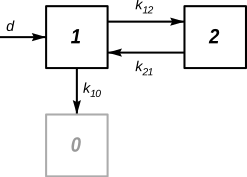
\includegraphics[width=0.275\textwidth]{img/perguntas/P1/P1-modelo-compartimental.png}
    \caption{Modelo compartimental \textcolor{gray}{(Imagem: Guia Laboratorial)}.}
    \label{fig:P1-modelo-compartimental}
\end{wrapfigure}

\vphantom{1}

A farmacocinética (PK) é responsável por determinar o destino das substâncias administradas no organismo e, portanto, os perfis\footnotemark[1] de tempo de concentração de substâncias no corpo. 

Tomando uma \textit{mechanistic modeling}\cite{teles_2017}, consideramos o modelo PK exposto (constantes definidas no Guia\scalebox{0.7}{$^{*^**}$}):
\vspace{-0.35em}\begin{equation}
    \begin{bmatrix}
        \dot{c_1} \\
        \dot{c_2}
    \end{bmatrix} =
    \begin{bmatrix}
        \frac{1}{V_1}(-K_{12}-K_{10}) & \frac{1}{V_1}K_{21}\\
        \frac{1}{V_2}K_{12} & -\frac{1}{V_2}K_{21}
    \end{bmatrix}
    \begin{bmatrix}
        c_1\\
        c_2
    \end{bmatrix} +
    \begin{bmatrix}
        \frac{1}{V_1}\\
        0
    \end{bmatrix}\delta d
\end{equation}

%%% BEGIN TABULAR
\vspace{-1em}
\begin{tabular}{c c}%%
    \hspace*{-1em}\noindent\begin{minipage}[t]{0.475\textwidth}
        \begin{lstlisting}[title=Pergunta 1 - Modelo PK (método de Euler),frame=tlrb]{P1}
%% Define variables
% (...)
%% Create f function -> c(t)' = f(c,d)
f = @(c,d)[
    (1/V*(-K12-K10)*c(1,:)+1/V*K21*c(2,:)+delta/V*d);
    (1/V*K12*c(1,:) - 1/V*K21*c(2,:))];
%% P1
Euler(f,t,h,d,size);
function Euler(f,t,h,d,size)
    % Preallocation
    c = zeros(2,size-1); 
    % Simple Euler's integration
    for i = 1:(size-1)
        c(:,i+1) = c(:,i) + h*f(c(:,i),d(i));
    end
    % Plot PK
    figure(), plot(t,c(1,:)), hold on; 
    plot(t,c(2,:)), plot(t,d);
    % (...)
end
        \end{lstlisting}
    \end{minipage} &\
    \noindent\begin{minipage}[t]{0.5\textwidth}
        \begin{figure}[H]
            \hspace*{-1.25em}
            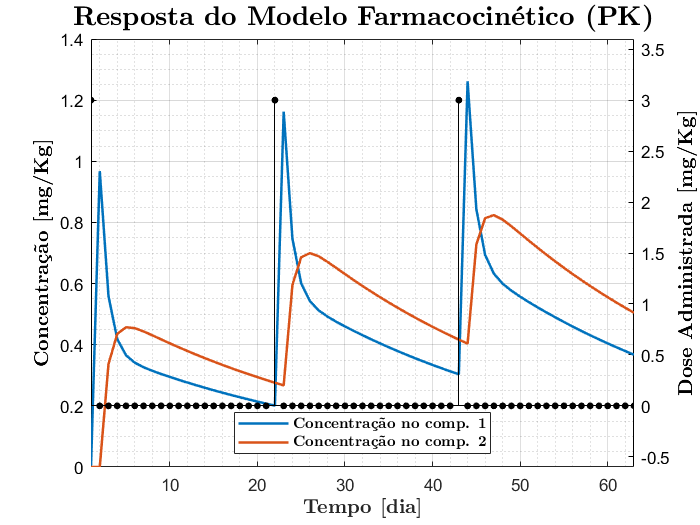
\includegraphics[width = 1\linewidth]{img/perguntas/P1/P1-PK.png}
            \caption{Concentrações nos compartimentos \textcolor{blue}{1} e \textcolor{orange}{2},\\ e dose administrada com um período de $T=21$d.}
            \label{fig:P1-modelo-PK}
        \end{figure}
    \end{minipage}
\end{tabular}
%%% END TABULAR

\vspace{1em}
Verifica-se que a administração de uma dose do fármaco, aumenta rapidamente $c_1$, correspondendo à \underline{fase de absorção} do medicamente pelo organismo. Em seguida,  observa-se a \underline{fase de distribuição}, em que a substância é distribuída ao longo do corpo, entranhando-se na(s) zona(s) de atuação, o que corresponde à diminuição de $c_1$ e aumento de $c_2$. Esta variação é proeminente logo após a administração, uma vez que a diferença de concentrações se verifica mais acentuada. A terceira fase observada corresponde à \underline{fase de excreção/metabolismo} do organismo, onde ambas as concentrações diminuem.
%//==============================--@--==============================//%
\footnotetext[1]{Estes perfis dependem de uma panóplia de fatores relacionados com propriedades da substância e à forma como o organismo reage inerentemente a esta; bem como do método de administração.\cite{teles_2017}}
